% \title{Apunte de Matemáticas Discretas CC3101:\\ 
% Representación, subgrafos, isomorfismos y conectividad de grafos  Clase 18}
% % \title{Ejercicios Lógica e Inducción}
% \author{Andrés Abeliuk}
% \date{}
% \maketitle


\section{Representación de grafos}

Una vez que comprendemos la noción abstracta de grafo, surge una pregunta natural: ¿cómo podemos representar un grafo en un computador de manera que sea útil para analizarlo y procesarlo? 
Existen varias formas de representar un grafo, y la elección depende del tipo de operaciones que queremos realizar sobre él.

La representación elegida puede afectar considerablemente la eficiencia de los algoritmos. Por ejemplo, encontrar los vecinos de un nodo es muy eficiente en una lista de adyacencia, pero verificar si dos nodos están conectados es inmediato en una matriz de adyacencia. 


Consideremos el siguiente grafo simple, no dirigido, con cuatro v\'ertices:
\begin{figure}[h]
\centering
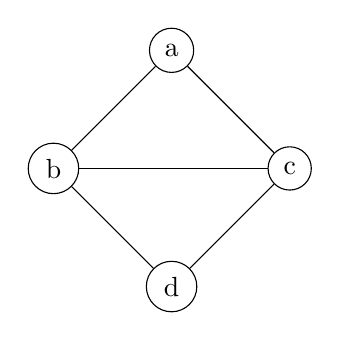
\begin{tikzpicture}[scale=1, every node/.style={circle, draw}]
  \node (a) at (0,1.5) {a};
  \node (b) at (-1.5,0) {b};
  \node (c) at (1.5,0) {c};
  \node (d) at (0,-1.5) {d};
  \draw (a) -- (b);
  \draw (a) -- (c);
  \draw (b) -- (d);
  \draw (c) -- (d);
  \draw (c) -- (b);
\end{tikzpicture}
\caption{Grafo base utilizado en las representaciones}
\label{fig:grafo-representaciones}
\end{figure}

Este grafo tiene:
\begin{itemize}
  \item V\'ertices: $V = \{a, b, c, d\}$
  \item Aristas: $E = \{(a,b), (a,c), (b,d), (c,d), (b,c)\}$
\end{itemize}
A continuaci\'on presentamos tres formas comunes para representar un grafo.

\subsection{Listas de adyacencia}

Una de las representaciones más comunes es la de \textbf{listas de adyacencia}, donde para cada vértice se mantiene una lista de sus vértices adyacentes.

\begin{definitionblock}{Lista de adyacencia}
Dado un grafo \( G = (V, E) \), una lista de adyacencia asocia a cada vértice \( v \in V \) un conjunto o lista de vértices adyacentes a \( v \), es decir, aquellos vértices \( u \in V \) tales que \( (v, u) \in E \).
\end{definitionblock}

\begin{exampleblock}{Ejemplo: Lista de adyacencia}
Lista de adyacencia correspondiente al grafo de la Figura~\ref{fig:grafo-representaciones}:
\begin{center}
\begin{tabular}{l|l}
V\'ertice & Adyacentes \\
\hline
a & b, c \\
b & a, c, d \\
c & a, b, d \\
d & b, c \\
\end{tabular}
\end{center}
\end{exampleblock}

Esta representación es eficiente en espacio cuando el grafo es \emph{disperso} (pocas aristas en relación al número de vértices).

\subsection{Matriz de adyacencia}

Otra forma clásica es la \textbf{matriz de adyacencia}, una matriz cuadrada de tamaño \( n \times n \), donde \( n = |V| \), que indica si existe una arista entre dos vértices.

\begin{definitionblock}{Matriz de adyacencia}
Sea \( G = (V, E) \) con \( V = \{v_1, v_2, \ldots, v_n\} \). La matriz de adyacencia \( A = [a_{ij}] \) se define como:
\[
a_{ij} =
\begin{cases}
1 & \text{si } (v_i, v_j) \in E \\
0 & \text{si } (v_i, v_j) \notin E
\end{cases}
\]
\end{definitionblock}

\begin{exampleblock}{Ejemplo: Matriz de adyacencia}
Matriz de adyacencia del grafo de la Figura~\ref{fig:grafo-representaciones}, en el orden \( a, b, c, d \):
\[
A = \begin{bmatrix}
0 & 1 & 1 & 0 \\
1 & 0 & 1 & 1 \\
1 & 1 & 0 & 1 \\
0 & 1 & 1 & 0
\end{bmatrix}
\]
\end{exampleblock}

Una propiedad interesante es que la matriz depende del orden de los vértices. Por tanto, un mismo grafo puede tener \( n! \) matrices distintas asociadas.

\subsection{Matriz de incidencia}

La tercera representación que estudiaremos es la \textbf{matriz de incidencia}, que vincula vértices con aristas.

\begin{definitionblock}{Matriz de incidencia}
Sea \( G = (V, E) \) con \( V = \{v_1, \ldots, v_n\} \) y \( E = \{e_1, \ldots, e_m\} \). La matriz de incidencia \( B = [b_{ij}] \) es una matriz \( n \times m \) donde:
\[
b_{ij} =
\begin{cases}
1 & \text{si el vértice } v_i \text{ es incidente en la arista } e_j \\
0 & \text{si no}
\end{cases}
\]
\end{definitionblock}

\begin{exampleblock}{Ejemplo: Matriz de incidencia}
Matriz de incidencia correspondiente al grafo de la Figura~\ref{fig:grafo-representaciones}, ordenando las aristas como: \( e_1 = (a,b), e_2 = (a,c), e_3 = (b,d), e_4 = (c,d), e_5 = (b,c) \):
\[
B = \begin{bmatrix}
1 & 1 & 0 & 0 & 0 \\
1 & 0 & 1 & 0 & 1 \\
0 & 1 & 0 & 1 & 1 \\
0 & 0 & 1 & 1 & 0
\end{bmatrix}
\]
\end{exampleblock}

Esta representación se utiliza frecuentemente en teoría de flujo y optimización lineal sobre redes.

\subsection*{Resumen y comparación}

\begin{center}
\resizebox{\textwidth}{!}{%
\begin{tabular}{l|c|c|c}
\textbf{Representaci\'on} & \textbf{Espacio} & \textbf{\'Eficiente para grafos densos?} & \textbf{\'Eficiente para grafos dispersos?} \\
\hline
Lista de adyacencia & \( O(n + m) \) & No & \textbf{S\'i} \\
Matriz de adyacencia & \( O(n^2) \) & \textbf{S\'i} & No \\
Matriz de incidencia & \( O(n \cdot m) \) & Intermedia & Intermedia \\
\end{tabular}
}
\end{center}

% \begin{quote}
% \textit{Curiosidad hist\'orica:} Las primeras matrices de adyacencia fueron utilizadas por el matem\'atico h\'ungaro D\'enes K\H{o}nig en su tratado pionero sobre teor\'ia de grafos en 1936.
% \end{quote}



\section{Subgrafos e Isomorfismo}

\subsection{Subgrafos}

En muchos casos, no es necesario considerar la totalidad de un grafo para resolver un problema. Basta con trabajar con una parte o ``fragmento'' de este.

\begin{definitionblock}{Subgrafo}
Sea $G = (V, E)$ un grafo. Un \textbf{subgrafo} de $G$ es un grafo $G' = (V', E')$ tal que $V' \subseteq V$ y $E' \subseteq E$. Decimos que el subgrafo es \textbf{propio} si $G' \neq G$.
\end{definitionblock}

\begin{exampleblock}{Ejemplo:}
En la Figura se muestra un grafo y un subgrafo resaltado en azul a su derecha.

\centering

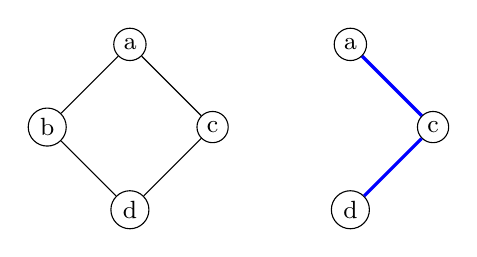
\begin{tikzpicture}[scale=0.7, every node/.style={circle, draw, inner sep=2pt, font=\small}]

  % Grafo original
  \node (a) at (0,1.5) {a};
  \node (b) at (-1.5,0) {b};
  \node (c) at (1.5,0) {c};
  \node (d) at (0,-1.5) {d};
  \draw (a) -- (b);
  \draw (a) -- (c);
  \draw (c) -- (d);
  \draw (b) -- (d);

  % Subgrafo
  \node (a2) at (4,1.5) {a};
  \node (c2) at (5.5,0) {c};
  \node (d2) at (4,-1.5) {d};
  \draw[blue, very thick] (a2) -- (c2);
  \draw[blue, very thick] (c2) -- (d2);
\end{tikzpicture}
\end{exampleblock}

\subsection{Isomorfismo de grafos}

A veces dos grafos tienen distinta \emph{apariencia}, pero representan esencialmente la misma estructura. En tales casos decimos que los grafos son \textbf{isomorfos}.

\begin{definitionblock}{Isomorfismo}
Sean $G = (V,E)$ y $G' = (V',E')$ dos grafos simples. Decimos que $G$ y $G'$ son \textbf{isomorfos} si existe una biyecci\'on $f \colon V \to V'$ tal que para todo par de v\'ertices $v_1,v_2 \in V$, se cumple:
\[
(v_1,v_2) \in E \quad \text{si y s\'olo si} \quad \bigl(f(v_1),f(v_2)\bigr) \in E'
\]
A la funci\'on $f$ se le llama un \textbf{isomorfismo} entre $G$ y $G'$.
\end{definitionblock}

\begin{exampleblock}{Ejemplo:}
\begin{minipage}{0.45\textwidth}
A continuaci\'on se muestran dos grafos que, aunque visualmente diferentes, son isomorfos.
\end{minipage}%%
\hfill
\begin{minipage}{0.4\textwidth}
\centering
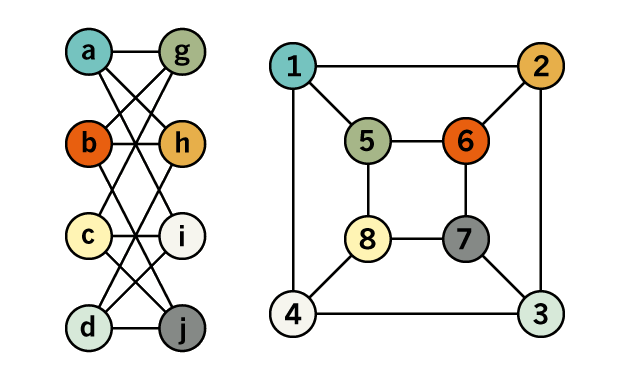
\includegraphics[width=\textwidth]{Figures/Isomorphism.png}
\end{minipage}
\end{exampleblock}


\begin{quote}
\textbf{Pregunta:} \textit{\'Cu\'antas posibles correspondencias (biyecciones) existen entre dos grafos simples con $n$ nodos?}
\end{quote}


\subsection{Demostrando isomorfismo y no isomorfismo}


Demostrar que dos grafos son isomorfos implica encontrar una biyecci\'on entre sus v\'ertices que preserve las adyacencias. Aunque conceptualmente directo, este problema es \textbf{computacionalmente costoso}. Los mejores algoritmos actuales para grafos generales tienen una complejidad \textbf{exponencial} en el n\'umero de v\'ertices. Por ello, es un problema central en el \textit{Graph Isomorphism Problem}, uno de los pocos problemas importantes cuya complejidad a\'{u}n no se conoce con certeza. 

La dificultad inherente en el problema de grafos isomorfos lo hacen un entretenido y desafiante puzzle:
\url{https://aabeliuk.github.io/graph-isomorphism-game/}


\subsubsection{Demostrando que dos grafos no son isomorfos}



\begin{exampleblock}{Ejemplo}
\textit{¿Són los siguientes grafos isomorfos?}
\begin{center}
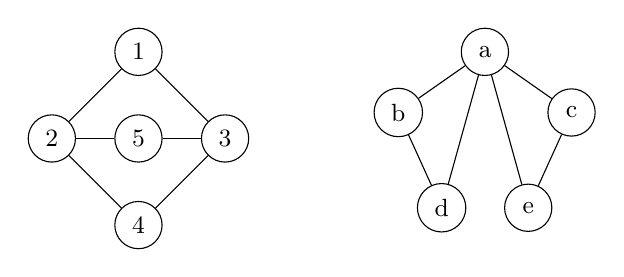
\begin{tikzpicture}[scale=1.1, every node/.style={circle, draw, minimum size=6mm, font=\small}]
  % Grafo G
  \node (g1) at (0,1) {1};
  \node (g2) at (-1,0) {2};
  \node (g3) at (1,0) {3};
  \node (g4) at (0,-1) {4};
  \node (g5) at (0,0) {5};
  \draw (g1) -- (g2);
  \draw (g1) -- (g3);
  \draw (g2) -- (g4);
  \draw (g3) -- (g4);
  \draw (g5) -- (g2);
  \draw (g5) -- (g3);

  % Grafo H
  \node (h1) at (4,1) {a};
  \node (h2) at (3,0.3) {b};
  \node (h3) at (5,0.3) {c};
  \node (h4) at (3.5,-0.8) {d};
  \node (h5) at (4.5,-0.8) {e};
  \draw (h1) -- (h2);
  \draw (h1) -- (h3);
  \draw (h1) -- (h4);
  \draw (h1) -- (h5);
  \draw (h2) -- (h4);
  \draw (h3) -- (h5);
\end{tikzpicture}
\end{center}

\medskip

\textbf{Respuesta:} No, porque uno de los grafos  tiene un v\'ertice de grado 4 (el v\'ertice $a$), mientras que el otro grafo no tiene ning\'un v\'ertice con ese grado.
\end{exampleblock}



\medskip

Para demostrar que dos grafos \textbf{no} son isomorfos, basta encontrar una \textbf{propiedad invariante} bajo isomorfismos que difiera entre ambos. Algunas propiedades invariantes comunes son:

\begin{itemize}
  \item N\'umero de v\'ertices y aristas.
  \item Grado de los v\'ertices.
  \item Existencia de ciclos de ciertas longitudes.
  \item Distribuci\'on de componentes conexas.
\end{itemize}

Estas invariantes permiten descartar el isomorfismo sin necesidad de revisar todas las permutaciones posibles.


\subsubsection{Clases de isomorfismo}

\begin{thmblock}{Isomorfismo es clase de equivalencia}
Demostrar que la relaci\'on de isomorf\'ia entre grafos define una relaci\'on de equivalencia en la colecci\'on de todos los grafos.

\textbf{Hint:} Demostrar que la relaci\'on es reflexiva, sim\'etrica y transitiva.
\end{thmblock}



\medskip

Dado que el isomorfismo de grafos es una relaci\'on de equivalencia, divide el conjunto de todos los grafos en \textbf{clases de equivalencia}.
No importa cu\'al de los grafos isom\'orficos de una clase de equivalencia se escoja: todos comparten la misma estructura esencial.

\textbf{Aplicaciones:} Esta idea de clasificar grafos en clases de isomorfismo tiene múltiples aplicaciones en distintas áreas. Permite representar moléculas como grafos y detectar compuestos equivalentes. En \textbf{bases de datos de grafos}, se utiliza para identificar duplicados estructurales, incluso si los nombres de los nodos difieren. En \textbf{reconocimiento de patrones}, ayuda a comparar estructuras como árboles sintácticos o redes neuronales. Finalmente, en \textbf{algoritmos}, permite optimizar procedimientos al operar sobre representaciones canónicas de clases de grafos equivalentes.

\subsubsection{Ejercicios sobre isomorfismo}

El \textbf{complemento} de un grafo simple $G = (V,E)$ es el grafo $\overline G = (V,\overline E)$, tal que
\[(v_1,v_2) \in \overline{E} \Leftrightarrow (v_1,v_2) \not \in E.\]
Un grafo simple es \textbf{auto-complementario} si $G$ es isomorfo a $\bar G$.

\begin{itemize}
  \item \textbf{Ejercicio:} Demuestre que el siguiente grafo es auto-complementario.
  \begin{center}
  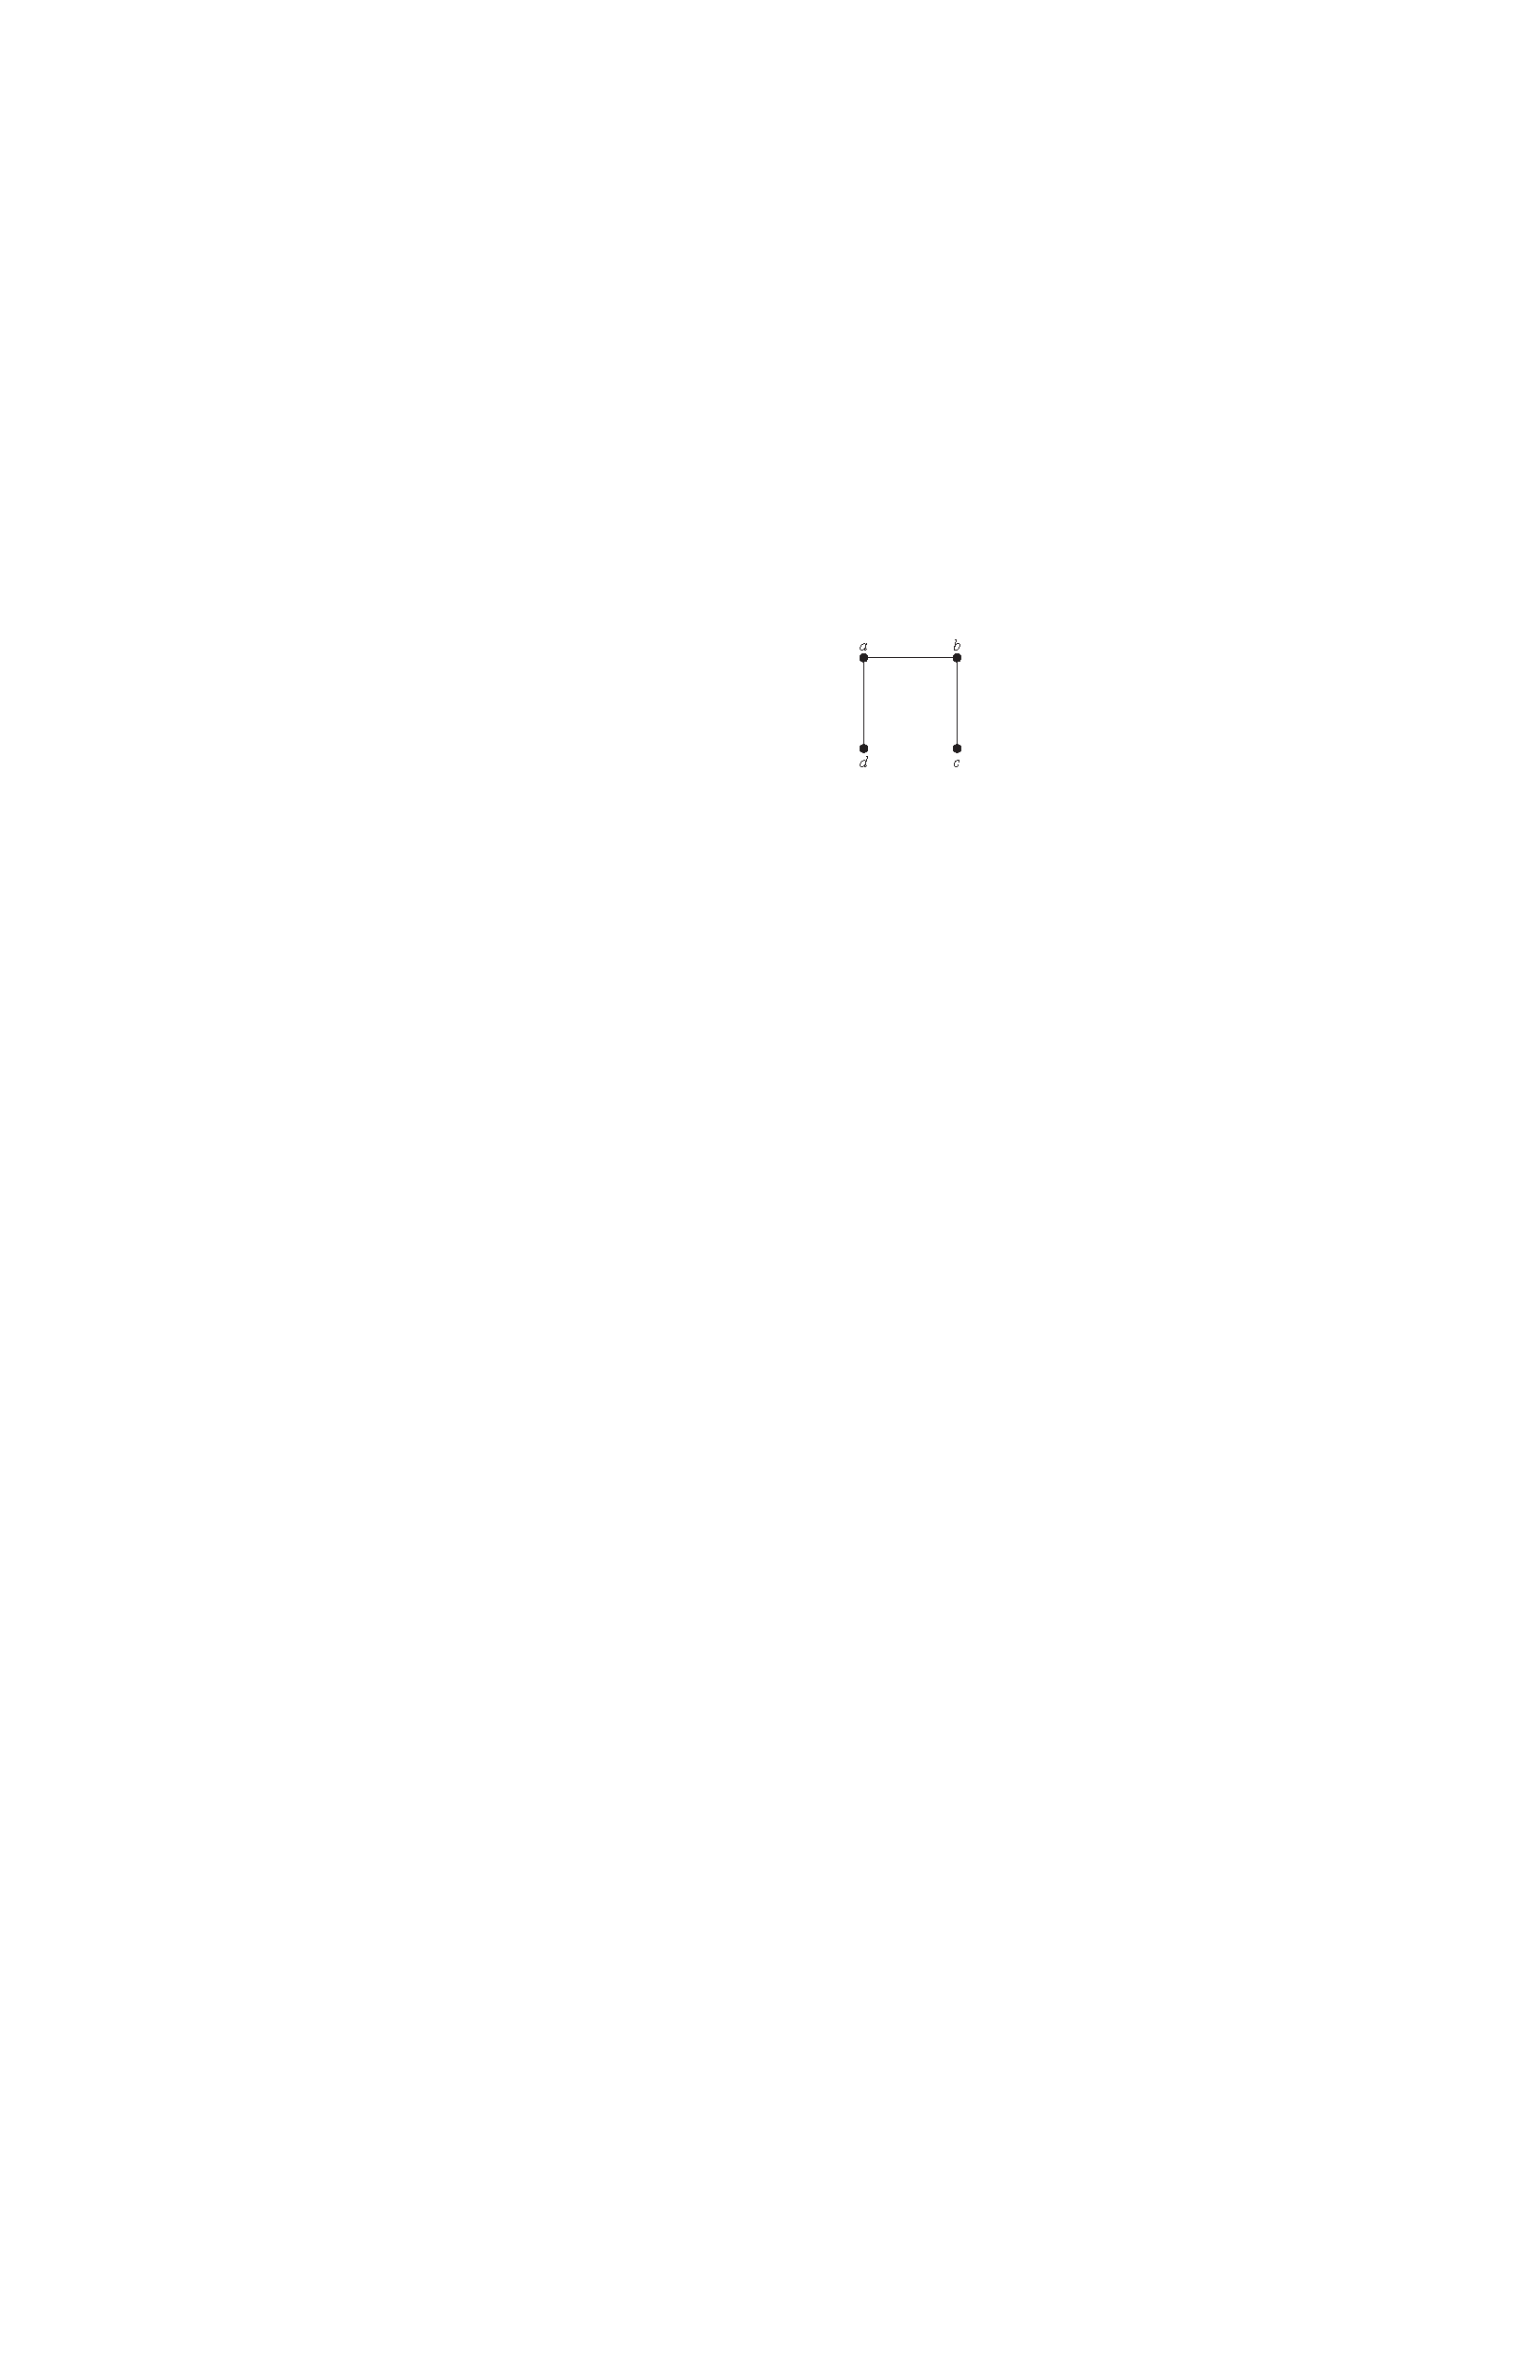
\includegraphics[width=0.15\textwidth]{Figures/SelfComplementary.pdf}
  \end{center}

  \item \textbf{Ejercicio:} Encuentre un grafo auto-complementario con 5 v\'ertices.

  % \item \textbf{Ejercicio:} \textquestiondown Para cu\'ales enteros $n$, el ciclo $C_n$ es auto-complementario?

  \item \textbf{Ejercicio:} Demuestre que si $G$ es un grafo auto-complementario simple con $n$ v\'ertices, entonces $n \equiv 0$ o $n \equiv 1$ m\'odulo 4.

 \item \textbf{Ejercicio:} ¿Cuántos grafos no isomorfos de 4 vértices existen? Dibújelos todos y justifique por qué no hay más.

\end{itemize}



\section{Caminos en grafos}

\subsection{Navegando grafos}

Muchos problemas pueden modelarse y resolverse \textbf{navegando grafos}. La noción de \textbf{camino} nos permite formalizar preguntas relacionadas con conectividad, eficiencia de recorrido y planificación de rutas.

\begin{itemize}
  \item \textbf{Ejemplo:} ¿Es posible mandar un mensaje entre dos computadoras usando las conexiones intermedias? Este problema puede resolverse explorando los caminos en una red.
  \item \textbf{Ejemplo:} ¿Cuál es la manera más rápida de salir de una granja, pasar por todos los establecimientos, y regresar al punto de partida? Esta es una instancia clásica del \textit{Problema del Viajante} (TSP).
\end{itemize}



\subsection{Definición de camino}

\begin{definitionblock}{Camino}
Sea $G = (V,E)$ un grafo no dirigido y sea $u,u' \in V$. Un \textbf{camino} (de largo $n$) entre $u$ y $u'$ es una secuencia de $n$ aristas $e_1, e_2, \ldots, e_n$ tal que existen nodos $v_0,v_1,v_2,\dots,v_n$ que satisfacen:
\begin{itemize}
  \item $v_0 = u$ y $v_n = u'$, y
  \item cada arista $e_i$ conecta $v_{i-1}$ y $v_i$, para $1 \leq i \leq n$
\end{itemize}
\end{definitionblock}

\begin{itemize}
  \item Si el camino no tiene aristas repetidas, se dice que es un \textbf{camino simple}.
  \item Si $u = u'$, entonces el camino se denomina \textbf{circuito} o \textbf{ciclo}.
\end{itemize}

\textbf{Notación:} Si el grafo no contiene aristas paralelas, podemos denotar un camino como la secuencia de vértices: $u,v_1,v_2,\ldots,v_{n-1},u'$.


\subsection{Conectividad de grafos no dirigidos}
En algunos grafos siempre es posible ir (i.e.~conectar mediante un camino) desde un vértice hasta cualquier otro. En otros no.

\begin{figure}[h!]
  \centering
  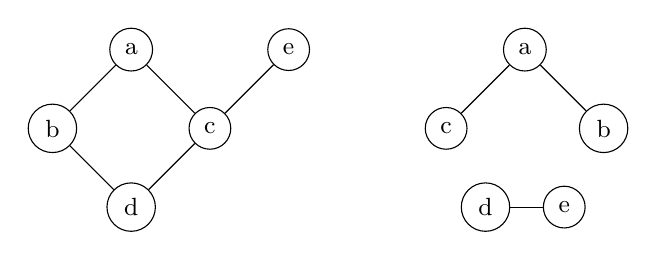
\begin{tikzpicture}[scale=1, every node/.style={circle, draw, minimum size=5mm, font=\small}]
    % Grafo conexo
    \node (a) at (0,1.5) {a};
    \node (b) at (-1,0.5) {b};
    \node (c) at (1,0.5) {c};
    \node (d) at (0,-0.5) {d};
    \node (e) at (2,1.5) {e};
    \draw (a) -- (b);
    \draw (a) -- (c);
    \draw (b) -- (d);
    \draw (c) -- (d);
    \draw (c) -- (e);

    % Separación
  
    % Grafo no conexo
    \node (f) at (5,1.5) {a};
    \node (g) at (6,0.5) {b};
    \node (h) at (4,0.5) {c};
    \draw (f) -- (g);
    \draw (f) -- (h);

    \node (i) at (4.5,-0.5) {d};
    \node (j) at (5.5,-0.5) {e};
    \draw (i) -- (j);
  \end{tikzpicture}
  \caption{Ejemplos de grafo conexo (izquierda) y no conexo (derecha)}
\end{figure}


\begin{definitionblock}{Conectividad}
Un grafo no dirigido se llama \textbf{conexo} sii existe un camino entre cada par de vértices distintos del grafo.
\end{definitionblock}

\begin{paragraph}{Propiedades e implicancias}
\leavevmode

Si existe un camino de $u$ a $v$ en un grafo $G = (V,E)$, entonces existe también un \textbf{camino simple} entre estos vértices. Esto es importante porque muchos algoritmos y teoremas operan sobre caminos simples, ya que descartan redundancias o ciclos intermedios.

Además, los caminos permiten definir \textbf{invariantes estructurales}, como la conectividad entre pares de vértices o la cantidad de componentes conexas. Estas invariantes pueden utilizarse para demostrar que dos grafos \textbf{no} son isomorfos, ya que todo isomorfismo debe preservar tales propiedades. Por ejemplo, si un grafo es conexo y otro no, no pueden ser isomorfos.
\end{paragraph}


\subsection{Componentes conexas}

Si un grafo es no conexo, entonces está formado por la unión disjunta de sus \textbf{componentes conexas}.

\begin{figure}[h]
  \centering
  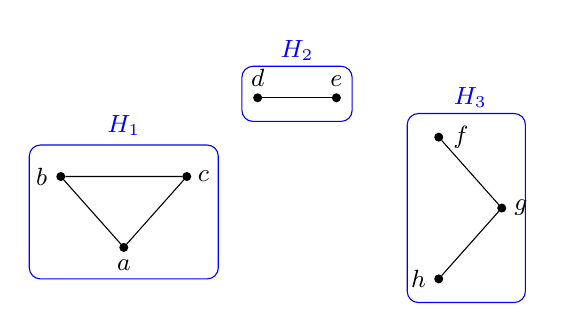
\begin{tikzpicture}[every node/.style={circle, draw, fill=black, inner sep=1pt}, font=\small]
    % Componente H1
    \node (a) at (1,-1)  [label=below:$a$] {};
    \node (b) at (0.2,-0.1) [label=left:$b$] {};
    \node (c) at (1.8,-0.1)  [label=right:$c$] {};
    \draw (a) -- (b) -- (c) -- (a);
    \draw[rounded corners, blue] (-0.2, -1.4) rectangle (2.2, 0.3);
    \node[draw=none, fill=none, text=blue] at (1,0.55) {$H_1$};

    % Componente H2
    \node (d) at (2.7,0.9)  [label=above:$d$] {};
    \node (e) at (3.7,0.9)  [label=above:$e$] {};
    \draw (d) -- (e);
    \draw[rounded corners, blue] (2.5, 0.6) rectangle (3.9, 1.3);
    \node[draw=none, fill=none, text=blue] at (3.2,1.5) {$H_2$};

    % Componente H3
    \node (f) at (5,0.4)  [label=right:$f$] {};
    \node (g) at (5.8,-0.5) [label=right:$g$] {};
    \node (h) at (5,-1.4) [label=left:$h$] {};
    \draw (f) -- (g);
    \draw (g) -- (h);
    \draw[rounded corners, blue] (4.6, -1.7) rectangle (6.1, 0.7);
    \node[draw=none, fill=none, text=blue] at (5.4, 0.9) {$H_3$};
  \end{tikzpicture}
  \caption{Ejemplo de grafo no conexo con tres componentes conexas $H_1$, $H_2$ y $H_3$}
\end{figure}



\begin{definitionblock}{Componente conexa}
Sea $G$ un grafo no dirigido. Una \textbf{componente conexa} de $G$ es un subgrafo $G'$ de $G$ tal que:
\begin{itemize}
  \item $G'$ es conexo, y
  \item $G'$ no es un subgrafo propio de otro subgrafo conexo de $G$.
\end{itemize}
En otras palabras, una componente conexa de $G$ es un subgrafo conexo \textbf{maximal}.
\end{definitionblock}

\subsection{Conectividad de grafos dirigidos}

Hay dos variantes de la noción de conectividad sobre grafos dirigidos: una considerando la dirección de los arcos y otra no. Para esta última, necesitamos la noción de grafo no-dirigido \textbf{subyacente}.

\begin{definitionblock}{Grafo no-dirigido subyacente}
Dado un grafo dirigido $G = (V,E)$, el \textbf{grafo no-dirigido subyacente} $G'$ de $G$ se obtiene a partir de $G$, computando la clausura simétrica de su conjunto de aristas $E$.
\end{definitionblock}

\begin{figure}[h!]
  \centering
  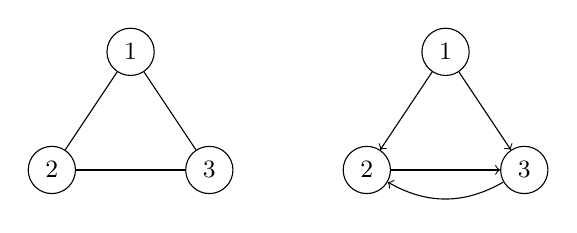
\begin{tikzpicture}[every node/.style={circle, draw, minimum size=6mm, font=\small}]
    % Grafo no dirigido (izquierda)
    \node (a) at (0,1.5) {1};
    \node (b) at (-1,0) {2};
    \node (c) at (1,0) {3};
    \draw (a) -- (b);
    \draw (a) -- (c);
    \draw (b) -- (c);

    % Grafo dirigido (derecha)
    \node (d) at (4,1.5) {1};
    \node (e) at (3,0) {2};
    \node (f) at (5,0) {3};
    \draw[->] (d) -- (e);
    \draw[->] (d) -- (f);
    \draw[->] (e) -- (f);
    \draw[->] (f) to[bend left] (e);
  \end{tikzpicture}
  \caption{Ejemplo de grafo no dirigido (izquierda) y grafo dirigido (derecha) con arcos entre nodos}
\end{figure}

\subsubsection{Conectividad fuerte y débil en grafos dirigidos}

\begin{definitionblock}{Conectividad en grafos dirigidos}
\begin{itemize}
  \item Un grafo dirigido es \textbf{fuertemente conexo} si para todo par de vértices $v, v'$, existe un camino dirigido de $v$ a $v'$ y viceversa.
  \item Un grafo dirigido es \textbf{débilmente conexo} si su grafo no dirigido subyacente es conexo, es decir, si para todo par $v, v'$ existe un camino entre ellos ignorando las direcciones.
\end{itemize}
\end{definitionblock}

\begin{figure}[h]
  \centering
  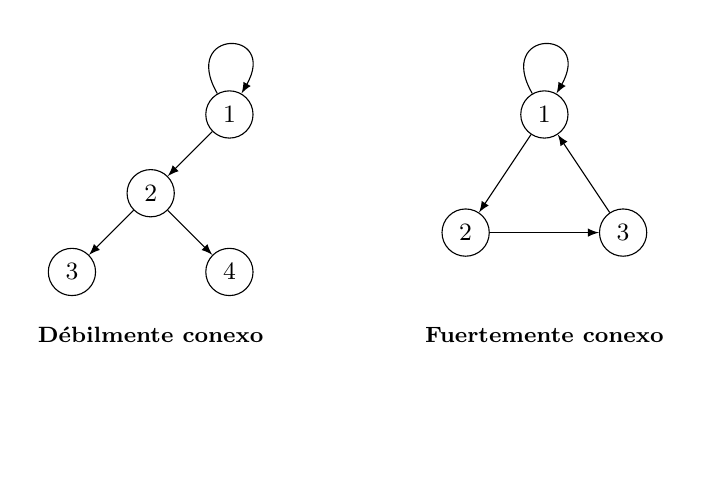
\begin{tikzpicture}[>=latex, every node/.style={circle, draw, minimum size=6mm, font=\small}]
    % Weakly connected graph
    \node (w1) at (0,2) {1};
    \node (w2) at (-1,1) {2};
    \node (w3) at (-2,0) {3};
    \node (w4) at (0,0) {4};
    \draw[->] (w1) to[out=120,in=60,loop] (w1);
    \draw[->] (w1) -- (w2);
    \draw[->] (w2) -- (w3);
    \draw[->] (w2) -- (w4);

    \node[draw=none] at (-1, -0.8) {{\footnotesize \textbf{Débilmente conexo}}};

    % Strongly connected graph
    \node (s1) at (4,2) {1};
    \node (s2) at (3,0.5) {2};
    \node (s3) at (5,0.5) {3};
    \draw[->] (s1) to[out=120,in=60,loop] (s1);
    \draw[->] (s1) -- (s2);
    \draw[->] (s2) -- (s3);
    \draw[->] (s3) -- (s1);

    \node[draw=none] at (4,-0.8) {{\footnotesize \textbf{Fuertemente conexo}}};
  \end{tikzpicture}
  \vspace{-4em}
  \caption{Comparación entre grafo débilmente conexo (izquierda) y fuertemente conexo (derecha)}
\end{figure}



\subsubsection{Componentes fuertemente conexas}

\begin{definitionblock}{Componente fuertemente conexa}
Sea $G$ un grafo dirigido. Una \textbf{componente fuertemente conexa} de $G$ es un subgrafo dirigido $G'$ tal que:
\begin{itemize}
  \item $G'$ es fuertemente conexo, y
  \item $G'$ no es un subgrafo propio de otro subgrafo fuertemente conexo de $G$.
\end{itemize}
\end{definitionblock}



\subsection{Caminos e isomorfismo}

La existencia de ciertos caminos también puede usarse como \textbf{invariante} para distinguir grafos no isomorfos.

\begin{exampleblock}{Ejemplo}
Utilice un invariante de caminos para demostrar que los grafos de la Figura~\ref{figure:ex_iso} no son isomorfos.

\medskip

\textbf{Respuesta:} Aunque los grafos tienen la misma cantidad de nodos y aristas, así como los mismos grados, el grafo $H$ tiene un circuito simple de largo 3 ($v_1,v_2,v_6,v_1$), mientras que $G$ no posee ninguno. Esto muestra que no pueden ser isomorfos.
\end{exampleblock}

\begin{figure}[h]
  \centering
  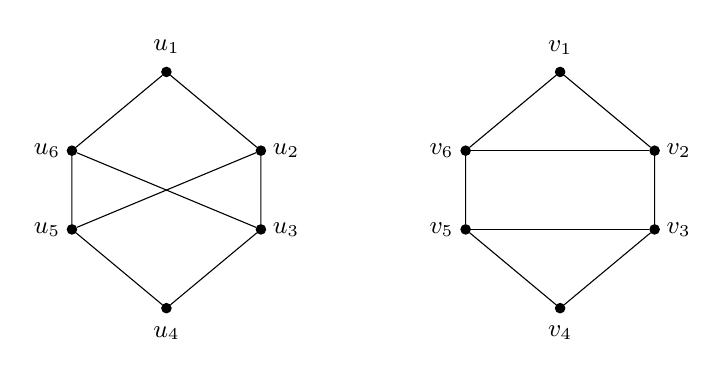
\begin{tikzpicture}[scale=1, every node/.style={circle, draw, fill=black, inner sep=1.2pt}, font=\small]
    % Grafo G
    \node (u1) at (0,2) [label=above:$u_1$] {};
    \node (u2) at (1.2,1) [label=right:$u_2$] {};
    \node (u3) at (1.2,0) [label=right:$u_3$] {};
    \node (u4) at (0,-1) [label=below:$u_4$] {};
    \node (u5) at (-1.2,0) [label=left:$u_5$] {};
    \node (u6) at (-1.2,1) [label=left:$u_6$] {};

    \draw (u1) -- (u2) -- (u3) -- (u4) -- (u5) -- (u6) -- (u1);
    \draw (u6) -- (u3);
    \draw (u2) -- (u5);
    % \node[draw=none]  at (0,-1.6) {\textcolor{cyan}{$G$}};
    

    % Grafo H
    \begin{scope}[xshift=5cm]
      \node (v1) at (0,2) [label=above:$v_1$] {};
      \node (v2) at (1.2,1) [label=right:$v_2$] {};
      \node (v3) at (1.2,0) [label=right:$v_3$] {};
      \node (v4) at (0,-1) [label=below:$v_4$] {};
      \node (v5) at (-1.2,0) [label=left:$v_5$] {};
      \node (v6) at (-1.2,1) [label=left:$v_6$] {};

      \draw (v1) -- (v2) -- (v3) -- (v4) -- (v5) -- (v6) -- (v1);
      \draw (v6) -- (v2);
      \draw (v5) -- (v3);
      % \node at (0,-1.6) {\textcolor{cyan}{$H$}};
    \end{scope}
  \end{tikzpicture}
  \caption{Dos grafos $G$ y $H$}
  \label{figure:ex_iso}
\end{figure}




\subsection{Ejercicios}

\begin{itemize}
  \item \textbf{Ejercicio:} Demuestre que para todo grafo conexo simple, todo nodo de grado impar está unido mediante un camino a algún otro nodo de grado impar.

  \item \textbf{Ejercicio:} Demuestre que todo grafo conexo con $n$ vértices debe tener al menos $n-1$ aristas.

  \item \textbf{Ejercicio:} Demuestre que un grafo simple $G$ es bipartito si y sólo si no contiene circuitos de largo impar.
\end{itemize}
